\documentclass[11pt,a4paper,oneside]{article}
\usepackage[UTF8,adobefonts]{ctex}

\usepackage{wrapfig}
\usepackage{indentfirst}
\usepackage{amsmath}
\usepackage{float}
\usepackage{ulem}
\usepackage[top=1in,bottom=1in,left=1.25in,right=1.25in]{geometry}

\usepackage{color}
\usepackage{xcolor}

\usepackage{multirow}

\begin{document}

\begin{figure}[H]
 \centering
  
\includegraphics[width=13cm]{表头.png}
\end{figure}
\begin{center}
\textbf{{\large 实验名称:\uline{          光的干涉实验1(分波面法) 激光双棱镜干涉       }}}
\end{center}

\section*{一、 实验重点}
\begin{enumerate}
 \item 熟练掌握采用不同光源进行光路等高共轴调节的方法和技术;
 \item 用实验研究菲涅耳双棱镜干涉并测定单色光波长;
 \item 学习用激光和其他光源进行实验时不同的调节方法。
\end{enumerate}

\section*{二、实验原理}

\subsection*{1.菲涅尔双棱镜干涉}
菲涅耳双棱镜可以看成是有两块底面相接、棱角很小的直角棱镜合成。若置单色光源S于双棱镜的正前方,则从S射来的光束通过双棱镜的折射后,变为两束相重叠的光,
这两束光仿佛是从光源S、的两个虚像S1和S2射出的一样。由于S1和S2是两个相干光源,所以若在两束光相重叠的区域内放置一个屏,即可观察到明暗相间的干涉条纹。

\begin{wrapfigure}{r}{0.4\textwidth}
  \vspace{-20pt}
  \begin{center}
    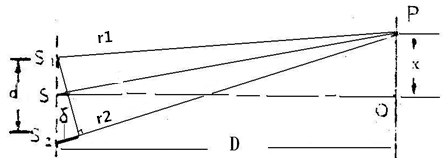
\includegraphics[width=0.48\textwidth]{ExperimentScience.png}
  \end{center}
  \vspace{-20pt}
  \vspace{-10pt}
\end{wrapfigure}

如图所示,设虚光源$S_1$和$S_2$的距离是d,D是虚光源到屏的距离。
令P为屏上任意一点,$r_1$和$r_2$分别为从$S_1$和$S_2$到P点的距离,
则从$S_1$和$S_2$发出的光线到达M点的光程差是:

\begin{center}
$\bigtriangleup$L= $r_2$-$r_1$
\end{center}

令$N_1$和$N_2$分别为$S_1$和$S_2$在屏上的投影,O为${N_1}{N_2}$的中点,
并设OP=x,则从${{\bigtriangleup}{S_1}{N_1}\text{P}}$及${\bigtriangleup}{S_2}{N_2}$P得:

\begin{center}
${r_1}^2=D^2+(x-{\displaystyle\frac{d}{2}})^2$
\end{center}

\begin{center}
${r_2}^2=D^2+(x+{\displaystyle\frac{d}{2}})^2$
\end{center}

两式相减,得:
\begin{center}
${r_2}^2-{r_1}^2=2dx$
\end{center}


另外又有${r_2}^2-{r_1}^2=({r_2}-{r_1})({r_2}+{r_1})={\bigtriangleup}L({r_2}+{r_1})$。通常D较d大的很多,所以${r_2}+{r_1}$近似等于2D,因此光程差为:

\begin{center}
${\bigtriangleup}L=\displaystyle\frac{dx}{D}$
\end{center}

如果$\lambda$为光源发出的光波的波长,干涉极大和干涉极小处的光程差是:

$$\Delta L=\frac{dx}{D}=
\left\{
\begin{aligned} 
k\lambda & (k=0,\pm 1,\pm2,...) \text{明纹}\\
 \displaystyle\frac{2k+1}{2}\lambda & (k=0,\pm 1,\pm2,...) \text{暗纹}\\
\end{aligned}
\right.
$$


由上式可知,两干涉条纹之间的距离是:

\begin{center}
$\Delta x=\displaystyle\frac{D}{d}\lambda$
\end{center}

所以用实验方法测得$\bigtriangleup$x,D和d后,即可算出该单色光源的波长:

\begin{center}
$\lambda =\displaystyle\frac{d}{D}{\Delta x}$
\end{center}

\subsection*{2.劳埃镜干涉}

\begin{figure}[htbp]
 \centering
  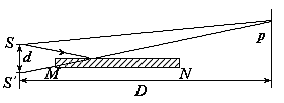
\includegraphics[width=10cm]{laoai.png}
\end{figure}

劳埃镜实验是由一块普通的平板玻璃构成的反射镜实现分波前干涉。单色光源S发出的光(波长为$\lambda$)以几乎掠入射的方式在平面镜MN上发生反射,反射光可以看做是在镜中的虚像S’发出的。S和S’发出的光波在其交迭区域发生干涉,可得条纹间距为:

\begin{center}
$\Delta x=\displaystyle\frac{D}{d}\lambda$
\end{center}
   
式中d为双光源S和S’间距,D为观察屏到光源的距离。

\section*{三、实验方案}

\subsection*{1.光源的选择} 
 当双棱镜与屏的位置确定之后,干涉条纹的间距△x与光源的波长λ成正比。为了获得清晰的干涉条纹,本实验采用单色光源,如激光、钠光等。

\subsection*{2.测量方法}
 条纹间距${\bigtriangleup}{x}$可直接用侧位目镜测出。虚光源间距d用二次成像的方法测130得:当保持物、屏位置不变
 且间距D大于4f时,移动透镜可在其间的两个位置成清晰的实像,一个是放大像,一个是缩小像。设b为虚光源缩小像间
 距,b’为放大像间距,则两虚光源的实际距离为$d=\sqrt{b{b}'}$,其中b和b’由测微目镜读出,同时根据两次成像
 的规律,若分别测出呈缩小像和放大像时的物距S、$S^’$,则物到像屏之间的距离$D=S+S^’$。根据波长的计算公式,得波长
 和各测量值之间的关系是:
 \begin{center}
 $\lambda =\displaystyle\frac{\Delta x\sqrt{b{b}'}}{S+{S}'}$\\
 \end{center}
 
\subsection*{3.光路组成}
\begin{wrapfigure}{r}{0.4\textwidth}
  \vspace{-20pt}
  \begin{center}
    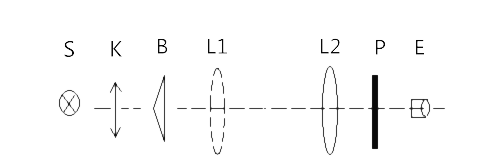
\includegraphics[width=0.48\textwidth]{Instrument1071.png}
  \end{center}
  \vspace{-20pt}
  \vspace{-10pt}
\end{wrapfigure}
 具体的光路如图所示,S为半导体激光器,K为扩束镜,B为双棱镜,P为偏振片,E为测微目镜。L为测虚光源间距d所用的凸透镜,透镜位于${L_1}$位置将使虚光源${S_1}{S_2}$在目镜处成方大像,透镜位于${L_2}$处将使虚光源在目镜出成缩小像。所有光学元件都放在光具座上,光具座上附有米尺刻度读出各元件的位置。
 
\section*{四、实验仪器}
   光具座,双棱镜,测微目镜,凸透镜,扩束镜,偏振片,白屏,可调狭缝,半导体激光器。
   
\section*{五、实验内容}

\subsection*{1.各光学元件的共轴调节}
\subsubsection*{1)调节激光束平行于光具座}
沿导轨移动白屏,观察屏上激光光点的位置是否改变,相应调解激光方向,直至在整根导轨上移动白屏时光点的位置不再变化,至此激光光束与导轨平行。
\subsubsection*{2)调双棱镜与光源共轴}
将双棱镜插于横向可调支座上进行调节,使激光点打在棱脊正中位置,此时双棱镜后面的白屏上应观察到两个等亮并列的光点,这两个光点的质量对虚光源像距b及b’的测量至关重要。此后将双棱镜置于距激光器约30cm的位置。
\subsubsection*{3)粗调测微目镜与其它元件等高共轴}
将测微目镜放在距双棱镜约70cm处,调节测微目镜,使光点穿过其通光中心。此时激光尚未扩束,决不允许直视测微目镜内的视场,以防激光坐灼伤眼睛。
\subsubsection*{4)粗调凸透镜与其他元件等高共轴}
将凸透镜插于横向可调支座上,放在双棱镜后面,调节透镜,使双光点穿过透镜的正中心。
\subsubsection*{5)用扩束镜使激光束变成点光源}
在激光器与双棱镜之间距双棱镜20cm处放入扩束镜并进行调节,使激光穿过扩束镜。在测微目镜前放置偏振片,旋转偏振片是测微目镜内视场亮度适中。
\subsubsection*{6)用二次成像法细挑凸透镜与测微目镜等高共轴}
通过“大像追小像”,不断调节透镜和测微目镜位置,直至虚光源大、小像的中心与测微目镜叉丝重合。
\subsubsection*{7)干涉条纹调整}
去掉透镜,适当微调双棱镜,使通过测微目镜观察到清晰的干涉条纹。

\subsection*{2.波长的测量}
\subsubsection*{1)测条纹间距${\bigtriangleup}$x}
连续测量20个条纹的位置${x_i}$ 。如果视场内干涉条纹没有布满,则可对测微目镜的水平位置略作调整;视场太暗可旋转偏振片调亮。
\subsubsection*{2)测量虚光源缩小像间距b及透镜物距S}
测b时应在鼓轮正反向前进时,各做一次测量。注意:i)不能改变扩束镜、双棱镜级测微目镜的位置;ii)用测微目镜读数时要消空程。
\subsubsection*{3)用上述同方法测量虚光源放大像间距b’及透镜物距S’。}
\end{document}
